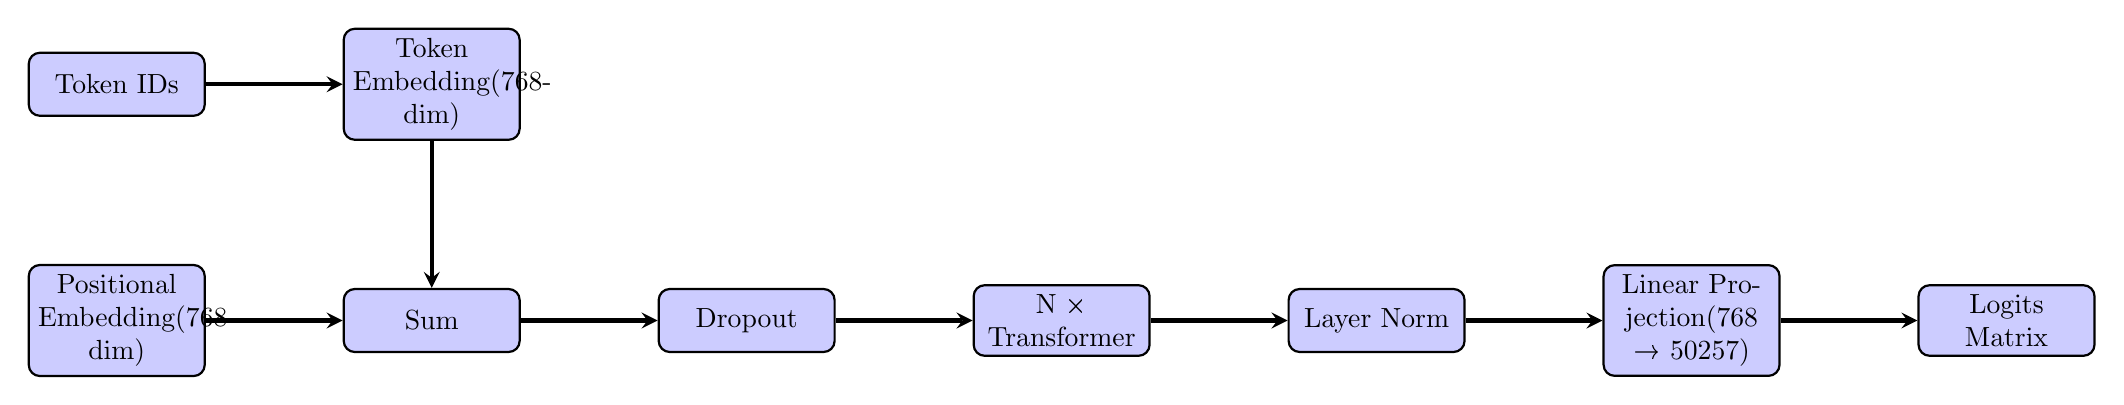
\begin{tikzpicture}[node distance=1.5cm, auto, thick]
  % Define styles
  \tikzstyle{block} = [rectangle, draw, fill=blue!20, text width=2cm, text centered, rounded corners, minimum height=0.8cm]
  \tikzstyle{arrow} = [draw, ->, >=stealth, line width=1.5pt]
  
  % Token IDs
  \node (tokenids) [block] {Token IDs};
  
  % Token Embedding Lookup
  \node (tokenemb) [block, right of=tokenids, xshift=2.5cm] {Token Embedding\n(768-dim)};
  \draw [arrow] (tokenids) -- (tokenemb);
  
  % Positional Embedding Lookup
  \node (posemb) [block, below of=tokenids, yshift=-1.5cm] {Positional Embedding\n(768-dim)};
  
  % Sum
  \node (sum) [block, right of=posemb, xshift=2.5cm] {Sum};
  \draw [arrow] (tokenemb) -- (sum);
  \draw [arrow] (posemb) -- (sum);
  
  % Dropout
  \node (dropout) [block, right of=sum, xshift=2.5cm] {Dropout};
  \draw [arrow] (sum) -- (dropout);
  
  % N × Transformer Blocks
  \node (transformer) [block, right of=dropout, xshift=2.5cm] {N × Transformer\nBlocks};
  \draw [arrow] (dropout) -- (transformer);
  
  % Layer Norm
  \node (layernorm) [block, right of=transformer, xshift=2.5cm] {Layer Norm};
  \draw [arrow] (transformer) -- (layernorm);
  
  % Linear Projection
  \node (linear) [block, right of=layernorm, xshift=2.5cm] {Linear Projection\n(768 → 50257)};
  \draw [arrow] (layernorm) -- (linear);
  
  % Logits
  \node (logits) [block, right of=linear, xshift=2.5cm] {Logits Matrix};
  \draw [arrow] (linear) -- (logits);
\end{tikzpicture}